\documentclass[english]{DESCARWINreport}

\usepackage{times}
\usepackage{helvet}
\usepackage{courier}
\usepackage{graphicx}
\usepackage{multirow}
%\usepackage[utf8]{inputenc}
\usepackage{algorithm}
\usepackage[noend]{algorithmic}
\usepackage{amsmath}
\usepackage{amsfonts}
\usepackage{amssymb}
\usepackage{array}
\usepackage{subfigure}
\usepackage{lscape}
%\usepackage{aaai}

\algsetup{indent=1.8em}
\renewcommand{\algorithmiccomment}[1]{// #1}
\newcommand{\pp}{planning tasks}
\newcommand{\PP}{planning task}
\newcommand{\dae}{{\em Divide-and-Evolve}}
\newcommand{\DAEI}{{\sc D\&E}}
\newcommand{\DAEII}{{\sc DaE2}}
\newcommand{\DAE}{{\sc DaE}}
\newcommand{\DAEX}{{\sc DaE$_{\text{X}}$}}
\newcommand{\DAEYAHSP}{{\sc DaE$_{\text{YAHSP}}$}}
\newcommand{\CPT}{{\sc CPT}}
\newcommand{\LPG}{{\sc LPG}}
\newcommand{\LAMA}{{\sc LAMA}}
\newcommand{\TFD}{{\sc TFD}}
\newcommand{\YAHSP}{{\sc YAHSP}}
\newcommand{\OPENSTACKS}{{\sc Openstacks}}
\newcommand{\ELEVATORS}{{\sc Elevators}}
\newcommand{\CREWPLANNING}{{\sc CrewPlanning}}
\newcommand{\FLOORTILE}{{\sc Floortile}}
\newcommand{\PARCPRINTER}{{\sc ParcPrinter}}


\def\UU{{\mathbb{U}}}

%\title{DESCARWIN\\\bigskip {\em \LARGE The Marriage of Descartes and Darwin}\\\bigskip \bigskip \bigskip \bigskip \bigskip \bigskip \bigskip {\LARGE WP1: the \DAEX\ Planning System}}
\title{DESCARWIN\\\bigskip {\em \LARGE The Marriage of Descartes and Darwin}\\\vspace{8cm} {\LARGE D5.4: Inoculation, Random Seeds and Variability}}
%ANR-09-COSI-002
%\author{Yann Semet}
\date{\today}
\laboratory{TRT - INRIA - ONERA}
\docref{62 441 217-179-6}

\revision{-}

%\setlength{\parindent}{0cm}
%\setlength{\parskip}{2ex plus 0.5ex minus 0.2ex}


% Pour réduire globalement l'espace entre les items d'une liste
% on peut également utiliser le bout de code suivant de M. Wooding
% Les paramètres utilisés pour définir cette mise en page
% sont les suivants :
% \topsep espace vertical supplémentaire (ajoute à \parskip)
% 	inséré entre le texte précédant la liste et le 1er objet
% 	de la liste
% \partosep espace vertical supplémentaire inséré devant la liste
% 	si celle-ci est précédée d'une ligne blanche
% \itemsep espace vertical supplémentaire (ajouté à \parsep)
% 	inséré entre les éléments d'une liste.

%%%% debut macro %%%%
\makeatletter
\toks@\expandafter{\@listI}
\edef\@listI{\the\toks@\setlength{\parsep}{0pt}}
\edef\@listI{\the\toks@\setlength{\topsep}{0pt}}
\makeatother
%%%% fin macro %%%%


\begin{document}

\maketitle

%\cleardoublepage

\begin{revisions}
\begin{revtable}
\dates{May 31, 2013}{}{}{}
\writers{Yann Semet\\Pierre Sav\'eant}{}{}{}
\approvers{P. Sav\'eant}{}{}{}
\end{revtable}
\begin{revisionlabels}
\revlabel{initial version}
\revlabel{}
\end{revisionlabels}
\end{revisions}

\begin{abstract}
This document provides the description and experimentation of work conducted to improve the initialization phase of DaE's evolutionary engine. We focus, in particular, on initialization procedures built around an individual provided either by specific construction or by invoking external planners. Following the biological metaphor inherent to evolutionary algorithms, such procedures are usually called "`artificial insemination"' or "`inoculation"' in the litterrature, we choose to stick to the latter. Three experimental campaigns are reported here. 

The first one is our early attempt at designing an inoculation procedure that builds the initial population around an individual constructed by our embeded planner, \YAHSP, with an additional routine designed to produce a consequently refined estimate of the critical parameter defining \YAHSP's exploratory allowance once the search has started, {$b_{max}$}. Experimental results show very poor performance and high risk of runs, with "`unlucky" random seeds, getting stuck in fruitless sampling of the search space. 

The second set of experiments follows a different strategy, getting rid of \YAHSP as the inoculant provider on one hand and being far more parsimonious with {$b_{max}$} on the other hand. We use additional sampling both to compensate for {$b_{max}$}'s restricted increase and to produce the inoculant. We call this procedure "`Inoculation through mass selection"'. Experimental results exhibit both substantial improvements in speed and risk reduction for our algorithm, albeit on a limited subset of the entire IPC benchmark. 

The third and final set of experiments reported here looks at how using external planners to provide the inoculant can be beneficial.
\end{abstract}

\tableofcontents

\newpage

\chapter{Introduction}

\begin{quotation}
\emph{"`It is difficult to catch a black cat in dark room, especially when it is not there."'}
\begin{flushright}
Chinese Proverb

\end{flushright}
\end{quotation}

\vspace{0cm}

\section{Context}

Search is about finding things that are difficult to locate. Stochastic search, evolutionary or otherwise, is about injecting randomness in the process when the field is so large or labyrinthine one has no other choice anyway. The challenge however, like the devil, is in the details of that randomness. There are many things one can do to improve one's odds of finding what one is looking for: throwing more light in, work in teams, use binoculars, ask someone, run faster, search deeper and so forth. All of these tricks have counterparts in mathematical optimization and computational search: local sampling, parallel search, depth first search, external expert knowledge, relaxed constraints, hybrid algorithms, etc. It all boils down to injecting whatever form of intelligence, knowledge or power is available at reasonable cost in the stochastic process to tame and steer randomness in the right direction.

Evolutionary algorithms offer many such avenues of improvement. They are usually made of many interconnected heuristically designed modules, each of which performing some portion of the traditional genetic loop with some flavor of randomness: initialization, selection, reproduction, blind variations, replacement, stopping criteria. Representation, helper or hybridized algorithms and genotype mappings can also benefit from efforts to build an intelligent bias for random search. \emph{DaE} makes no exception: it is an evolutionary algorithm coupled with an embedded AI planner. It has a convoluted workflow, five variation operators and dozens of parameters and routines, many of which have been designed or tuned with somewhat arbitrary randomness based ingredients which can be improved with externally provided intelligence.

In that perspective, the traditional evolutionary building block the present report deals with is \emph{initialization}. More specifically, we look at how the initial population, and therefore the entire algorithm, can be improved by being made less pointlessly random from the start. The idea is to find a way to start the search directly from an interesting zone instead of blindly sampling the search space as is usually done by default. One possible way to do this is known as \emph{inoculation}. In biology or medicine, inoculation refers to "`the placement of something that will grow or reproduce, and is most commonly used in respect of the introduction of a serum, vaccine, or antigenic substance into the body of a human or animal, especially to produce or boost immunity to a specific disease"'. In our mathematical context we will seek to find a way to quickly construct one individual with a good fitness value or good building blocks and use variations of that individual to constitute the initial population. That individual, which we will call the \emph{inoculant} will serve as the vehicle for the injection of interesting search space information into the genetic population where it will be spread and sampled along with successive generations.  Obviously enough, this process relies on the assumption that we can design a way to fabricate this individual both quickly enough and with enough interesting material for inoculation to be worth the extra cost in algorithmic terms.

To sum up, and come back to our metaphoric epigraph, we will henceforth try to catch the cat faster by starting at least from the right room.

\section{Rationale}


As mentionned earlier

Expert vs. black box


Dangers and tricks of the trade



Rationale (P1, P2, etc.)
\begin{description}

\item[Motivation 1 : bypassing "`crazy randomness"'] Moving from chaos to early order, especially around representation...

\item[Motivation 2 : precomputation, landmarks, initial quirks]

\item[Motivation 3 : solving a relaxed version of the problem]

\item[Motivation 4 : having a first shot at the actual problem]

\item[Motivation 5 : using algorithm portfolios]

\item[Motivation 6 : experts talking]

\item[Motivation 7 : statistics and sampling]

\end{description}

\section{State of the Art}

Messy GAs \cite{Kargupta95search}, PBIL \cite{Baluja95removingthe}, EDAs \cite{Larranaga:2002b}

Surry \cite{Surry96, SurryPhD}

Semet \cite{semetGECCO06}

\newpage
\chapter{Inoculation with Yahsp}

\section{Meet Adam!}

\subsection{Definition d'adam}

outline globale Initialization

\begin{algorithm}[h!]
\caption{generateIndividual(N)}
\label{algoInit}
{\small
\begin{algorithmic}[1]
\REQUIRE{$T$} \hfill \COMMENT{candidate start times}
\STATE{$D \leftarrow \{\}$}\hfill \COMMENT{ordered list of timestamps}
\REPEAT
\STATE{$t \leftarrow \UU(T)$} 
\STATE{$T \leftarrow T \setminus \{t\}$} 
\STATE{Insert($t,D)$} \hfill  \COMMENT{maintain $D$ ordered}
\UNTIL{$\#D = N$}
\STATE{$\text{Ind} \leftarrow \{\}$}  \hfill \COMMENT{start building the individual}
\FOR{$t \in \ D $}
\STATE{$s \leftarrow \{\}$} \hfill \COMMENT{start building the intermediate goal}
\STATE{$A_t \leftarrow \{a \in A\;|\;T(a) = t\}$}    \hfill \COMMENT{atoms that can appear at $t$}
\STATE{$n \leftarrow \UU([1,\#A_t])$} \hfill \COMMENT{number of atoms} \label{init.state}
\WHILE{$n \neq 0 \wedge A_t \neq \{\}$} \label{begin.loopInit}
\STATE{$a \leftarrow \UU(A_t)$}    \hfill \COMMENT{choose uniformly an atom in $A_t$}
\STATE{$s \leftarrow s \cup \{a\}$}   \hfill \COMMENT{add to $s$}
\STATE{$A_t \leftarrow A_t\setminus \left(\{a\} \cup M(a)\right)$ }  \hfill \COMMENT{remove all mutex}
\STATE{$n \leftarrow n-1$}
\ENDWHILE \label{end.loopInit}
\STATE{$\text{Ind} \leftarrow \text{Ind} + \{s\}$}  \hfill \COMMENT{add the new intermediate goal}
\ENDFOR
\RETURN{Ind}
\end{algorithmic}
}
\end{algorithm}


outline estimate bmax incremental

outline estimate bmax inoc


\subsection{Experiments}

Setup : pop 100, 10 minutes, ratio 1%, etc.

Results : avg plot (with vs without) + proportion frozen

Elevators

Openstacks

Floortiles





\section{Perturbations around Adam}


Rationale : seeing how Adam can be exploited

Plots : avg fitness variation with increasing mutation radius (first add adtom then add goal) + proportion of infeasible individuals

As one can in see in figure \ref{myLabel}, the results are speaking by themselves.

%\begin{figure}
%\begin{figure}[!t]
%\centering
%\includegraphics*[width=10cm,height=10cm]{bmax.png}
%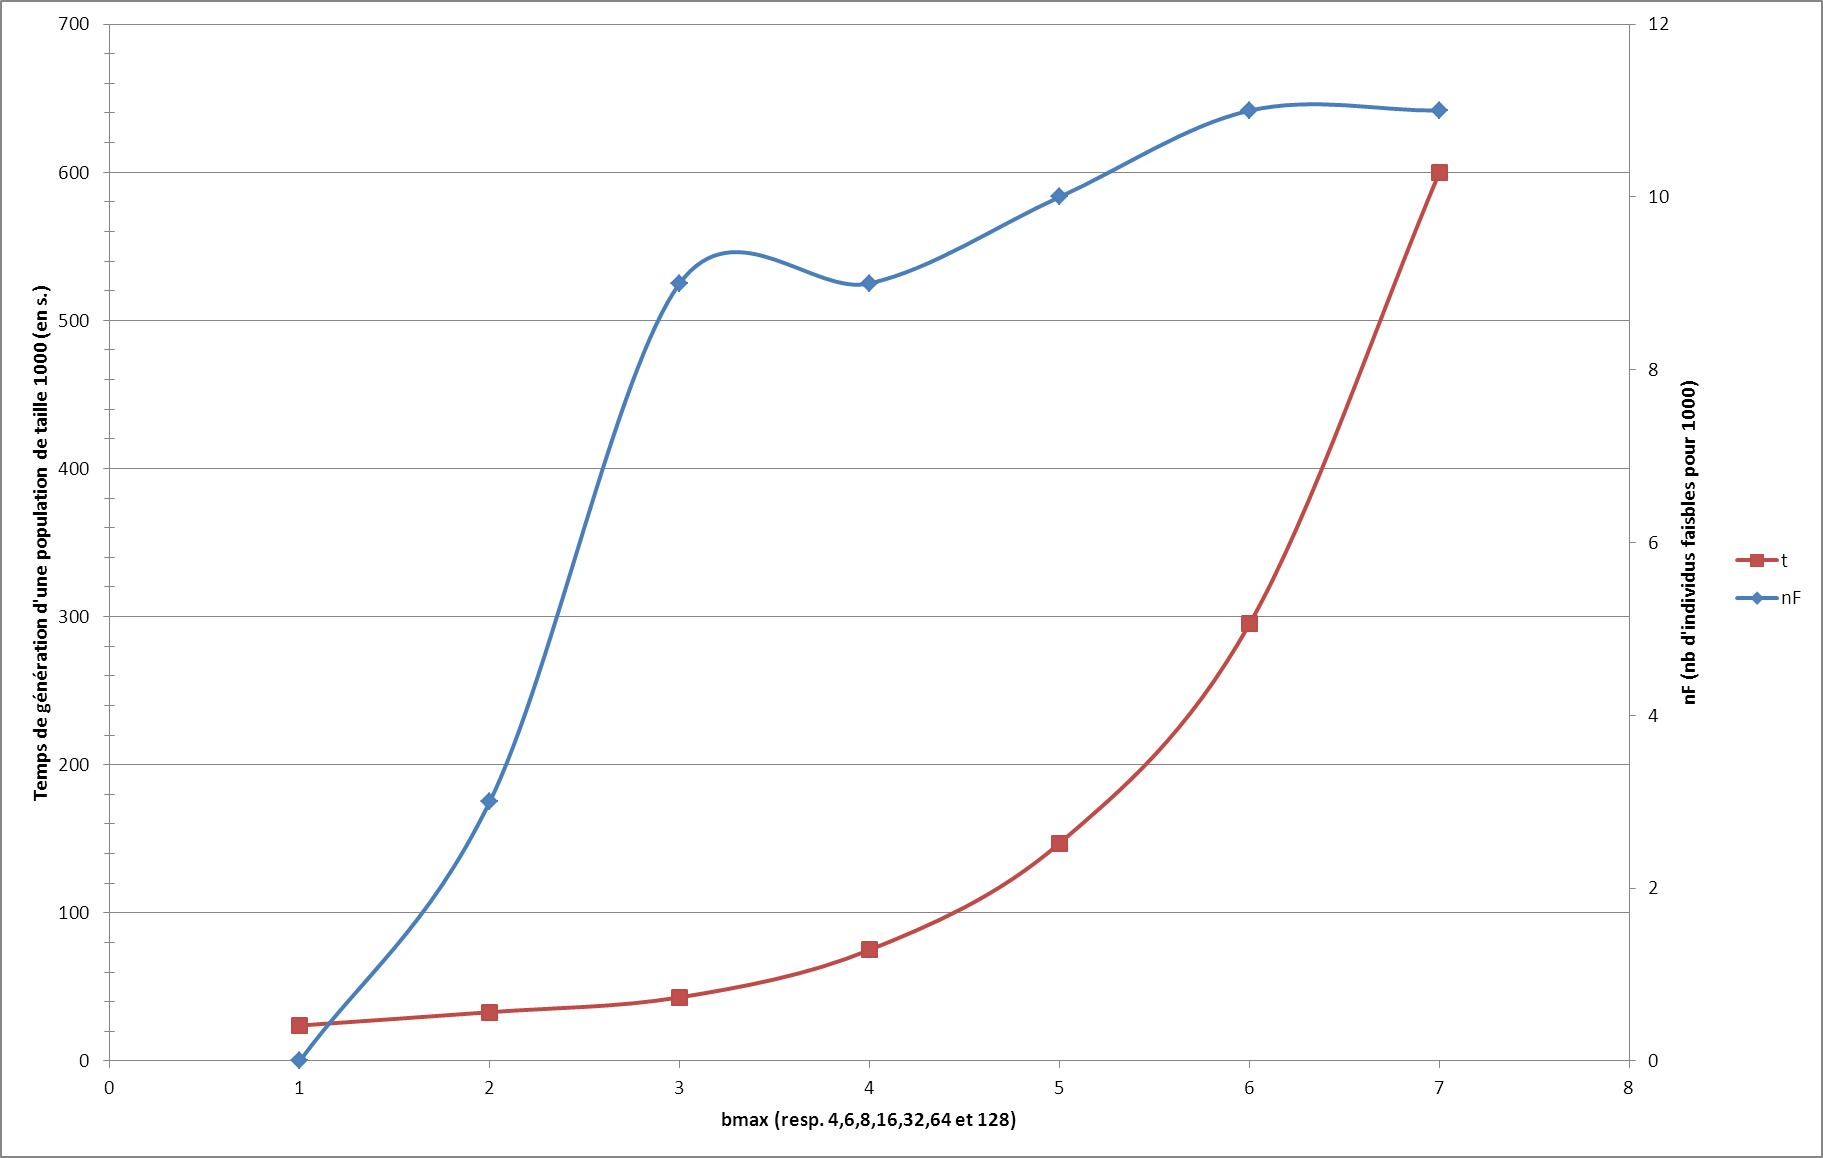
\includegraphics[scale=0.3]{bmax.png}
%\caption{this is the caption}
%\label{myLabel}
%\end{figure}


\begin{figure}
	\centering
		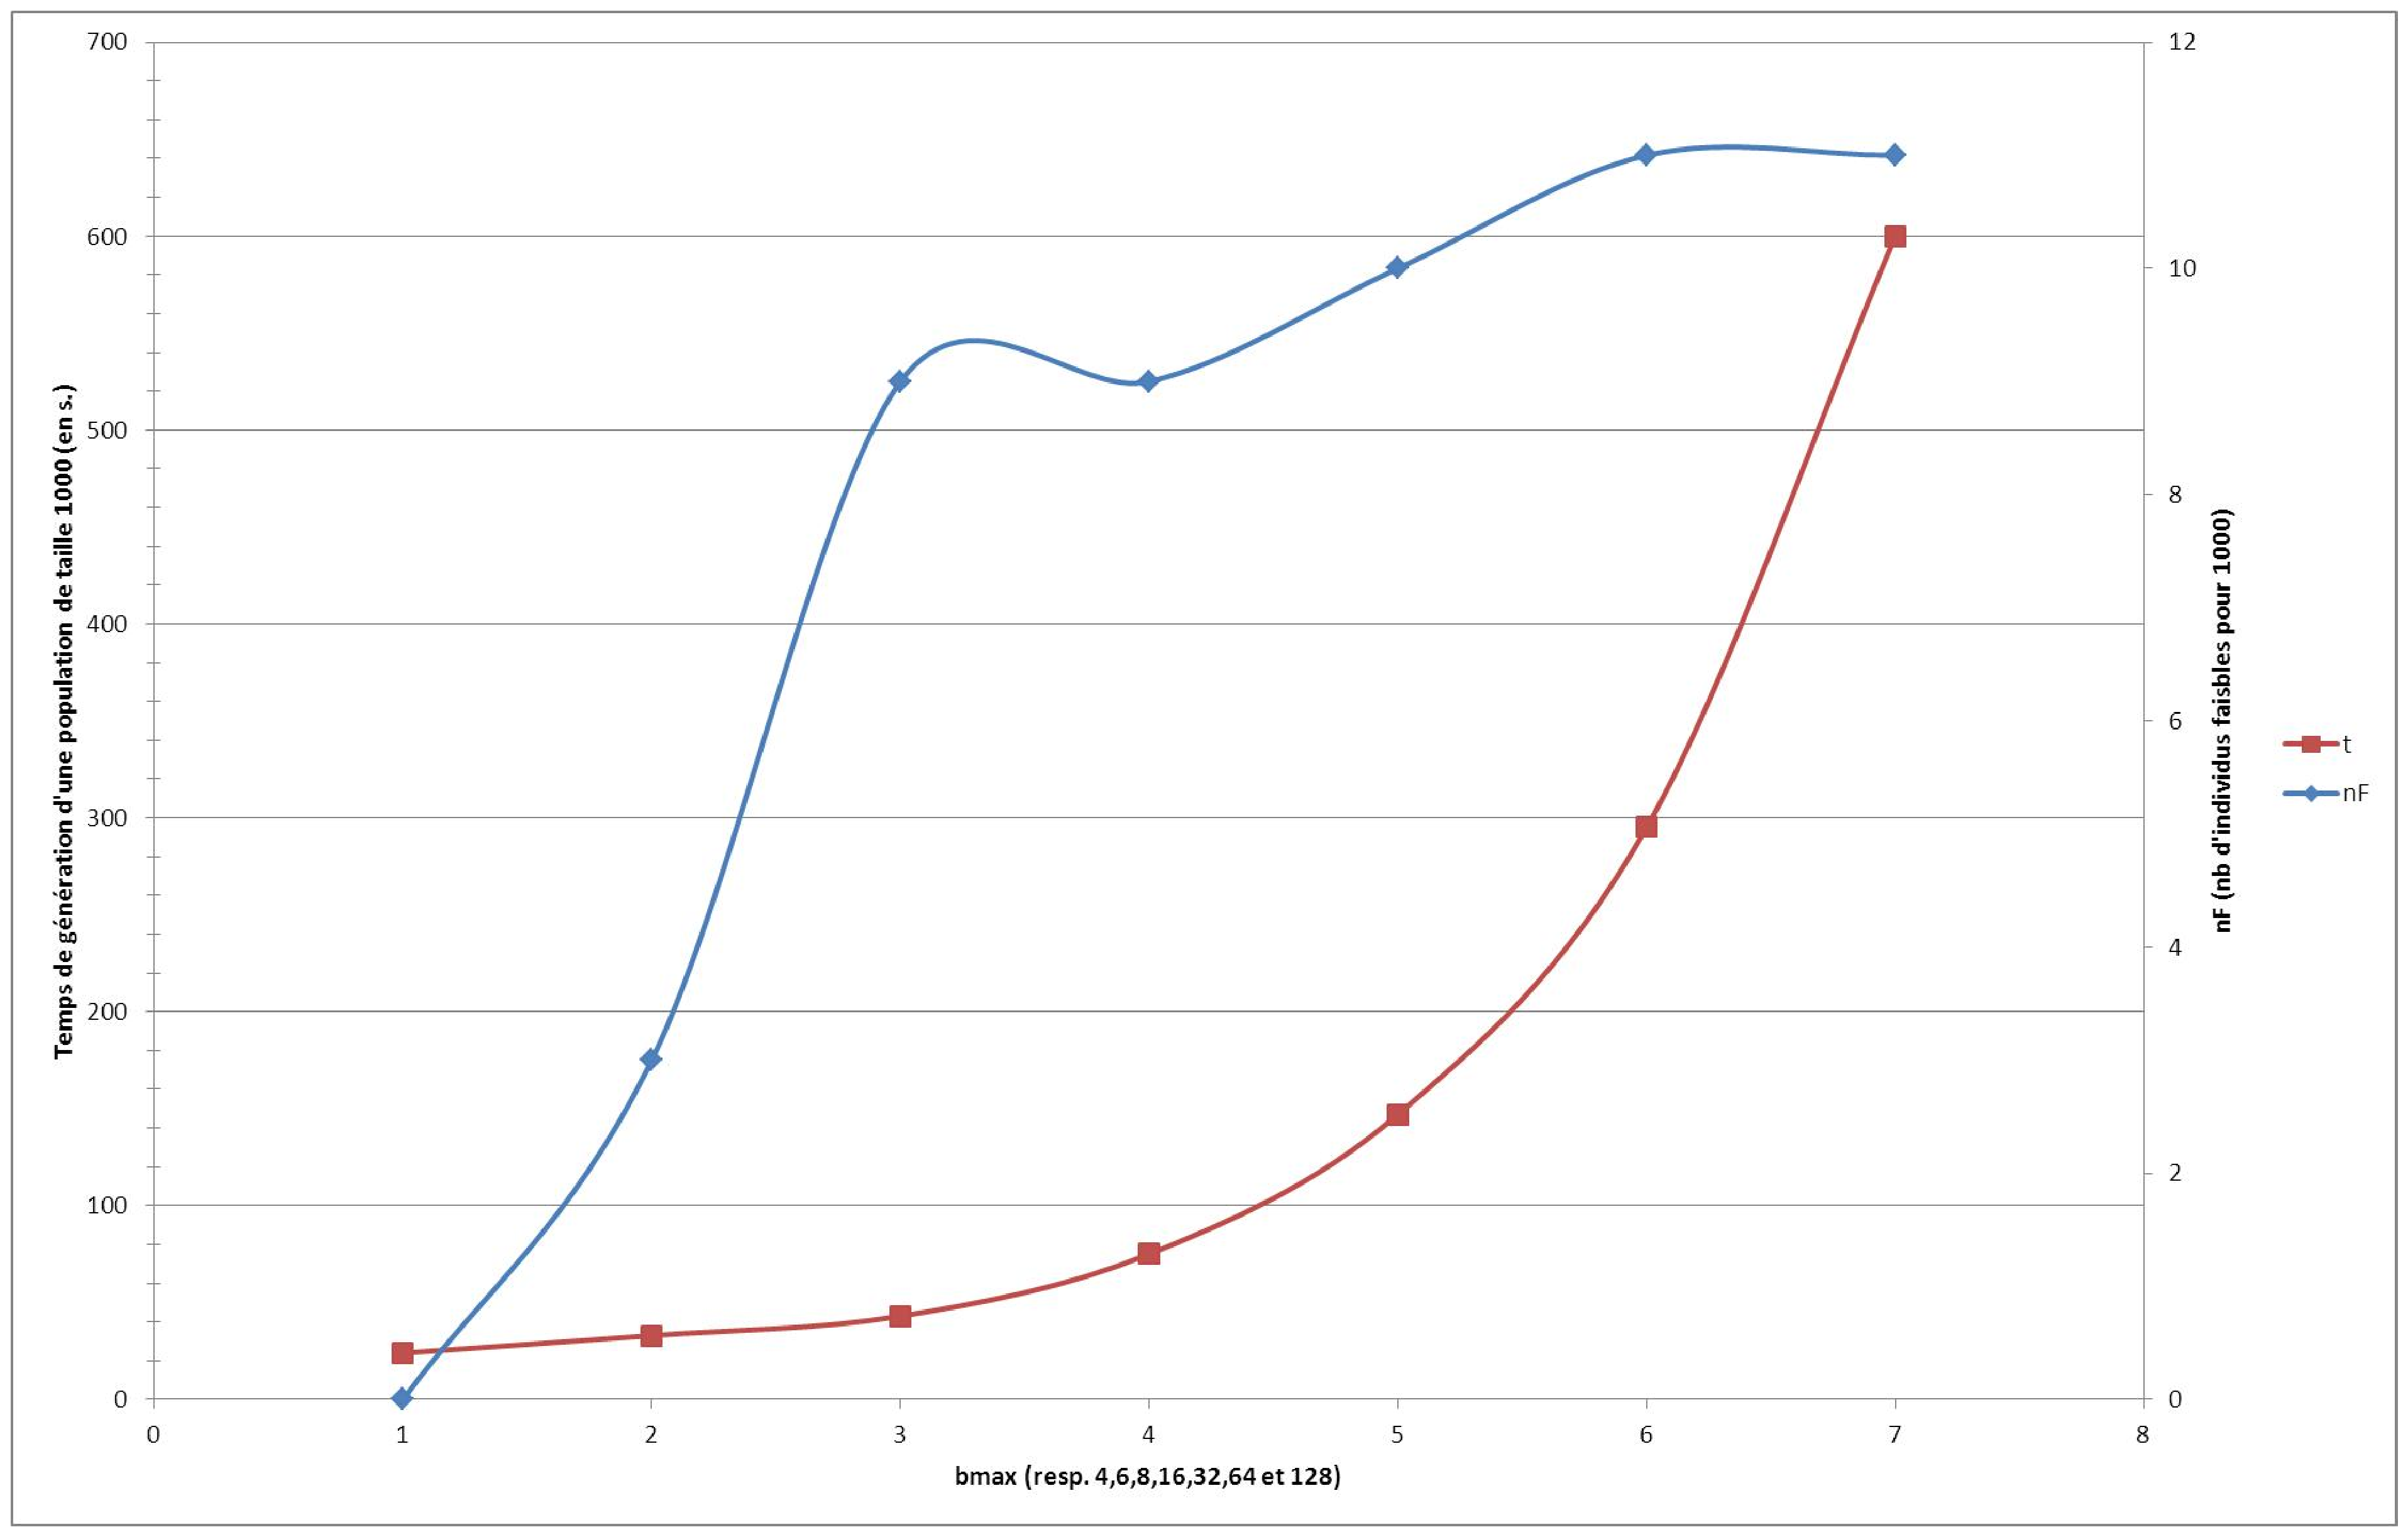
\includegraphics[width=0.9\textwidth]{pics/bmax.eps}
	\caption{hellooo}
	\label{fig:bmax}
\end{figure}


\chapter{Population sizing, extra sampling and risk reduction}

\section{The importance of bmax, proportion of lost runs}

plot : sector with bmax

plot : time lost vs. benefit

\section{Inoculation through mass selection}

plot : quality maintained
plot : avg over time 
indictators : proportion of lost runs and overall speed ratio


\section{Smaller populations}

undersampling vs speed


%\chapter{To Climb Or Not To Climb?}
%\section{Variance in YAHSP}
%\section{Replacement?}


\chapter{Inoculation with other planners}

\section{Lama, Popf2, Cpt And Others}

Inoculation benefit wrt time given to create inoculant



\chapter{conclusion}



\chapter{References}


\bibliographystyle{plain}
\bibliography{D_5_4}

%\begin{thebibliography}{}
%\bibliographystyle{plain}
%
%\bibitem{AligneSaveant2010}
%Aligne, F.; and Sav\'eant, P.
%\newblock Gestion de crise : optimisation de la mise en {\oe}uvre des plans de secours.
%\newblock In Workshop Interdisciplinaire sur la S{\'e}curit{\'e} Globale ({\em WISG 2010}).
%
%\end{thebibliography}



\end{document}


%\vspace{-0.2cm}
%\begin{algorithm}[h!]
%\caption{evaluate(Ind, planner)}
%\label{algoFitness}
%{\small
%\begin{algorithmic}[1]
%\REQUIRE{$I$, $G$, $b_\text{max}$, $l_\text{max}$}
%\STATE{$k \leftarrow 0 \; ; \; u \leftarrow 0 \; ; \; B \leftarrow 0$}
%\STATE{$i \leftarrow$ I$ \; ; \; g \leftarrow \{\}$}
%\WHILE{$g \neq G$} \label{begin.loop}
%\STATE{$g\leftarrow $ nextGoal(Ind)}
%\STATE{$(sol_k, b_{\text{done}}) \leftarrow \mbox{planner.Solve}(i,g,b_{\text{max}})$} \label{CPT.solve}
%\IF{$sol_k = \bot$} \label{CPT.fail}
%\RETURN {($\bot$, $10\cdot k \cdot \text{\it dist}(i,G) + \text{length(Ind)} - u)$} \label{return.infeasible}
%\ELSIF[\hfill avoid empty plan]{$\text{length}(sol_k) > 0$} \label{useful.states}
%\STATE{$u \leftarrow u+1$} \hfill \COMMENT{useful states counter}
%\STATE{$B \leftarrow B + b_{\text{done}}$} \hfill \COMMENT{total search steps} \label{algo-backtracks}
%\ENDIF
%\STATE{$i \leftarrow$ ExecPlan$(i,sol_k)$}  \hfill \COMMENT{next initial state}\label{global.state}
%\STATE{$k\leftarrow k+1$} \hfill \COMMENT{intermediate goal counter}
%\ENDWHILE \label{end.loop}
%\STATE{$(Sol, Q)\leftarrow \mbox{Compress}((sol_j)_{0 \leq j \leq k})$} \label{CPT.compress}
%\RETURN{$(Sol, Q+\frac{length(Ind)-u+1}{Q} + \frac{B}{l_\text{max} \cdot\, b_\text{max}})$} \label{return.feasible}
%\end{algorithmic}
%}
%\end{algorithm}
%\vspace{-0.2cm}
%
%\vspace{-0.2cm}
%\begin{algorithm}[h!]
%\caption{crossover(Ind$_1$,Ind$_2$)}
%{\small
%\label{algo-crossover}
%\begin{tabbing}
%1: $s_a$ \= $\leftarrow$ \= $\UU($Ind$_1)$ \` // Ind$_1 =(s_i)_{1 \leq i \leq n}$\\
%2: $t_b$ \> $\leftarrow$ \> $\UU($Ind$_2)$ \` // Ind$_2 =(t_i)_{1 \leq i \leq m}$\\
%3: {\bf if} $\Delta(t_b) > \Delta(s_a)$ \= {\bf then} \= {\bf return} \= $(s_1,\ldots,s_a,t_b,\ldots,t_m)$\\
%4: \> {\bf else} \> {\bf return} \> $(t_1,\ldots,t_b,s_a,\ldots,s_n)$
%\end{tabbing}
%}
%\vspace{-0.2cm}
%\end{algorithm}
%\vspace{-0.3cm}
%
%\vspace{-0.2cm}
%\begin{algorithm}[h!]
%\caption{addGoal(Ind)}
%\label{algo-addGoal}
%{\small
%\begin{algorithmic}[1]
%\REQUIRE{$r$} \hfill \COMMENT{neighborhood radius}
%\STATE{$j \leftarrow \UU$([1, min(length(Ind),lastReached(Ind))])}
%\STATE{$s\leftarrow \{\}$} \hfill \COMMENT{insert $s$ between $s_j$ and $s_{j+1}$}
%\STATE{$t \leftarrow \UU(\{t \in T\;|\; \Delta(s_j) < t \leq \Delta(s_{j+1}) \})$} %\hfill \COMMENT{$\Delta(s_j) < t \leq \Delta(s_{j+1})$}
%\STATE{$A_t \leftarrow \{a \in A \;|\; T(a)\in \text{neighbourhood}(t,r) \} $} 
%\STATE{$A_m\leftarrow \{\}$ } \hfill \COMMENT{set of non pairwise mutex atoms}
%\WHILE{$A_t\neq \{\}$}
%\STATE{$a \leftarrow \UU(A_t)$}
%\STATE{$A_m\leftarrow A_m\cup \{a\}$ }
%\STATE{$A_t \leftarrow A_t \setminus (\{a\}\cup M(a))$}
%\ENDWHILE
%\STATE{$N \leftarrow \UU([1,\#A_m])$} \hfill \COMMENT{goal length}
%\REPEAT 
%\STATE{$a \leftarrow \UU(A_m)$} \hfill \COMMENT{choose uniformly an atom in $A_m$}
%\STATE{$s \leftarrow s \cup \{a\}$} \hfill \COMMENT{add to $s$}
%\STATE{$A_m\leftarrow A_m \setminus \{a\}$}\hfill \COMMENT{remove from $A_m$ }
%\UNTIL{$\#s = N$}
%\STATE{insert(Ind, $s$, $j$)} \hfill \COMMENT{insert $s$ after goal j}
%\RETURN{Ind}
%\end{algorithmic}
%}
%\end{algorithm}
%\vspace{-0.3cm}
%
%\vspace{-0.2cm}
%\begin{algorithm}[h!]
%\caption{addAtom(Ind)}
%\label{algo-modifstateadd}
%{\small
%\begin{algorithmic}[1]
%\REQUIRE {$p_c, p_a$} \hfill \COMMENT{relative probabilities to change or add an atom}
%\FORALL{$k \in$ [1,min(length(\text{Ind}),lastReached(\text{Ind})+1)]}
%\IF[\hfill atom change]{$\UU([0,1]) < \frac{p_c}{\text{length(Ind)}}$}
%\STATE{$a \leftarrow \UU(\text{Ind}[k])$}
%\STATE{$b \leftarrow \UU(\{b \in M(a)\;|\;T(b)=\Delta(\text{Ind}[k]) \land \nexists c  \in \quad~\hskip 0.8cm (\text{Ind}[k] \setminus \{a\}), b \in M(c)\})$}
%\STATE{$\text{Ind}[k] \leftarrow (\text{Ind}[k] \setminus \{a\}) \cup \{b\}$}
%\ENDIF
%\IF[\hfill atom addition]{$\UU([0,1]) < p_a$}
%\STATE{$a \leftarrow \UU(\{b \in A\;|\; T(b) = \Delta(\text{Ind}[k]) \land \nexists c \in \quad~\hskip 1cm \text{Ind}[k], b \in M(c)\})$}
%\STATE{$\text{Ind}[k] \leftarrow \text{Ind}[k] \cup \{a\}$}
%\ENDIF
%\ENDFOR
%\RETURN{Ind}
%\end{algorithmic}
%}
%\end{algorithm}
%\vspace{-0.4cm}
%
%
%\vspace{-0.2cm}
%\vspace{-0.2cm}
%
%\begin{algorithm}[tb!]
%\caption{DAEX({\scriptsize popSize, OffSpringSize, MaxGen, MaxChgt,} {\small p$_\text{cross}$, p$_\text{mut}$, w$_\text{addGoal}$, w$_\text{delGoal}$, w$_\text{addAtom}$, w$_\text{delAtom}$, b$_\text{max}$, l$_\text{max}$, $r, p_c, p_a$})}
% {\scriptsize // Main loop: $h=h^1$ popSize=100, OffSpringSize = 700}}
%\label{algoMain}
%{\small
%\begin{algorithmic}[1]
%\REQUIRE{planner, $h$}\hfill \COMMENT{embedded planner and heuristic function}
%\FORALL{$a \in A$}
%\STATE{$T(a) \leftarrow h(a)$} \hfill \COMMENT{compute earliest start time}
%\ENDFOR
%\STATE{$T \leftarrow \{T(a) \neq 0\;|\;a \in A\}$} \hfill \COMMENT{candidate start times set}
%\STATE{pop $\leftarrow$ \{\}} \hfill \COMMENT{start building the population}
%\REPEAT
%\STATE{pop $\leftarrow$ pop $\cup$ \{GenerateIndividual($\UU([1,\#T])\}$)} \label{init.sequence}
%\UNTIL{$\#$pop = popSize}
%\REPEAT \label{main.loop}
%\STATE{offspring $\leftarrow$ \{\}}
%\REPEAT
%\STATE{Ind$_1$ $\leftarrow$ $\UU$(pop)}
%\IF{$\UU([0,1])$ $<$ p$_\text{cross}$}
%\STATE{Ind$_2$ $\leftarrow$ $\UU$(pop)}
%\STATE{Newind $\leftarrow$ crossover(Ind$_1$,Ind$_2$)}
%\ELSE
%\STATE{Newind $\leftarrow$ Ind$_1$}
%\ENDIF
%\IF{$\UU([0,1])$ $<$ p$_\text{mut}$}
%\STATE{$f \leftarrow$ $\UU_\text{weighted}$({\scriptsize addGoal, addAtom, delGoal, delAtom, w$_\text{addGoal}$, w$_\text{delGoal}$, w$_\text{addAtom}$, w$_\text{delAtom}$})}
%\STATE{Newind $\leftarrow$ APPLY($f$, Newind)}
%\ENDIF
%\STATE{offspring $\leftarrow$ offspring $\cup$ \{Newind\}}
%\UNTIL{$\#$offspring = OffSpringSize}
%\FORALL{Ind $\in$ pop $\cup$ offspring}
%\STATE{Evaluate(Ind, planner)}
%\ENDFOR
%\STATE{pop $\leftarrow$ SurvivalSelection(pop $\cup$ offspring)}\label{main.survival}
%\UNTIL{$\#$gen $>$ MaxGen OR noImprovementSince(MaxChgt)}
%\RETURN{Evaluate(pop.BestIndividual, planner).Sol}
%\end{algorithmic}
%}
%\end{algorithm}
